\subsubsection{Les actions utilisateurs}
Avec l'application {\nomApplication}, Utilisateur peut réaliser diverses actions :
\begin{itemize}
    \item Se reconnecter au programme {\nomLogiciel}.
    \item Démarrer et arrêter l'envoi de trames.
    \item Ajouter un objet.
    \item Supprimer un objet ou une trame.
    \item Déplier ou replier le menu de l'objet.
    \item Saisir une trame.
    \item Ajouter une trame.
    \item Arrêter ou relancer la réception des trames dans le sniffer.
    \item Revenir en haut du sniffer.
    \item Exporter les trames du sniffer.
    \item Supprimer les trames du sniffer.
\end{itemize}
\medskip
La figure \ref{ecran_boutons} montre le nom des boutons et des champs de texte de EcranPrincipal.
\begin{minipage}{1\linewidth}
    \centering
    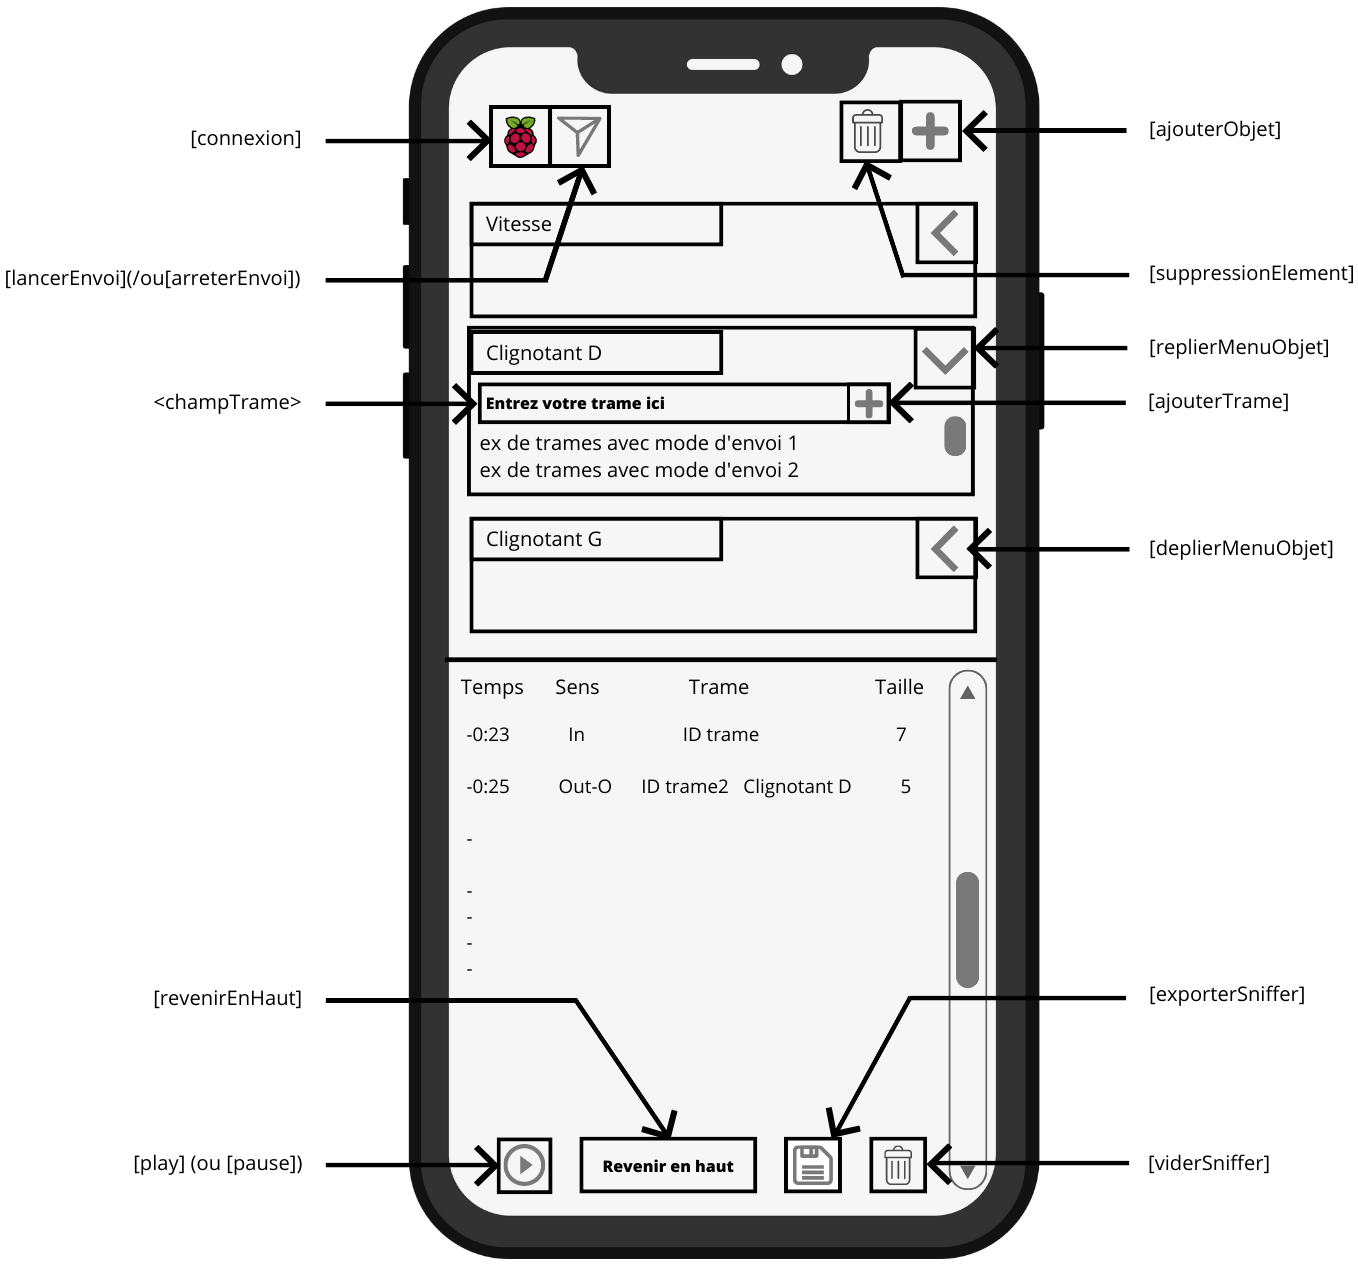
\includegraphics[width=0.85\textwidth]{sections/3_Exigences_specifiques/1_IHM/ihm/ecranPrincipalDescription.png}
    \captionof{figure}{EcranPrincipal avec légende des boutons et des champs}
    \label{ecran_boutons}
\end{minipage} \newline \medskip \medskip

L'ensemble des figures suivantes représente les noms des boutons et des champs de texte de tous les différents pop-up utilisés dans l'application {\nomApplication}. \\
\medskip

\begin{minipage}{1\linewidth}
    \centering
    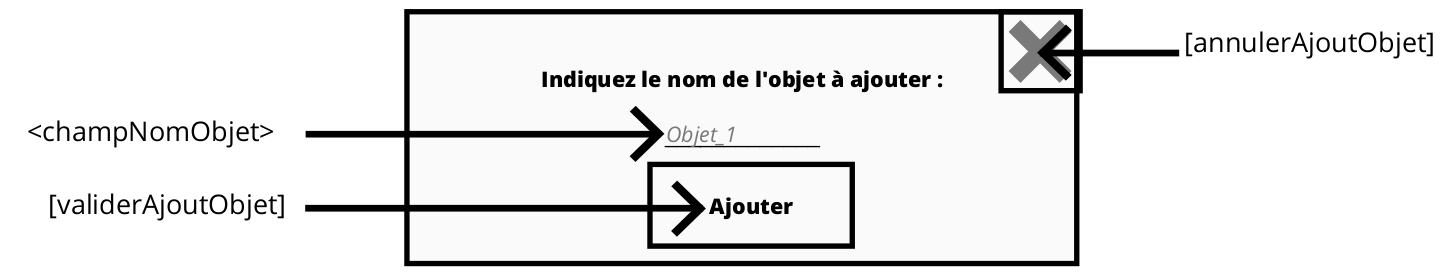
\includegraphics[width=0.91\textwidth]{sections/3_Exigences_specifiques/1_IHM/ihm/popUpObjet.png}
    \vspace{-0.3cm}
    \newline
    \captionof{figure}{PopupAjoutObjet avec nom des boutons et du champ de saisie}
    \label{ecran_ajout_objet}
\end{minipage} \newline
\vspace{1cm}

\begin{minipage}{1\linewidth}
    \centering
    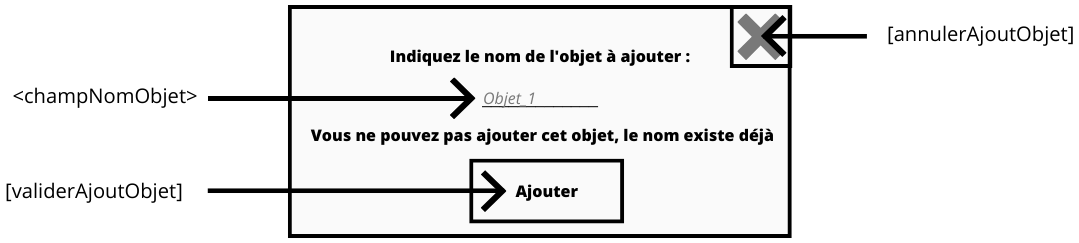
\includegraphics[width=0.91\textwidth]{sections/3_Exigences_specifiques/1_IHM/ihm/popupErreurSaisieObjet.png}
    \vspace{-0.3cm}
    \newline
    \captionof{figure}{PopupErreurAjoutObjet avec nom des boutons et du champ de saisie}
    \label{ecran_erreur_ajout_objet}
\end{minipage} \\ \\

\begin{minipage}{1.3\linewidth}
    \centering
    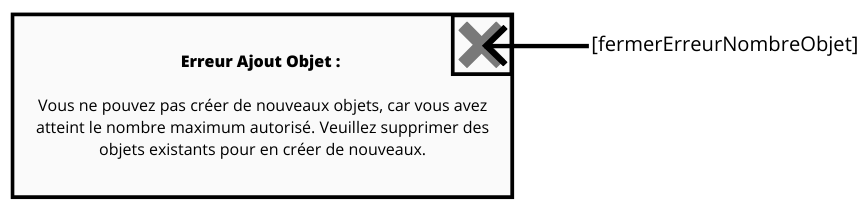
\includegraphics[width=0.66\textwidth]{sections/3_Exigences_specifiques/1_IHM/ihm/popUpErreurAjoutObjet.png}
    \captionsetup{justification=centering, margin={-5cm,0cm}}
    \captionof{figure}{PopupErreurNombreObjet avec nom du bouton}
    \label{ecran_erreur_ajout_nombre_objet}
\end{minipage}\\ \\

\begin{minipage}{1\linewidth}
    \centering
    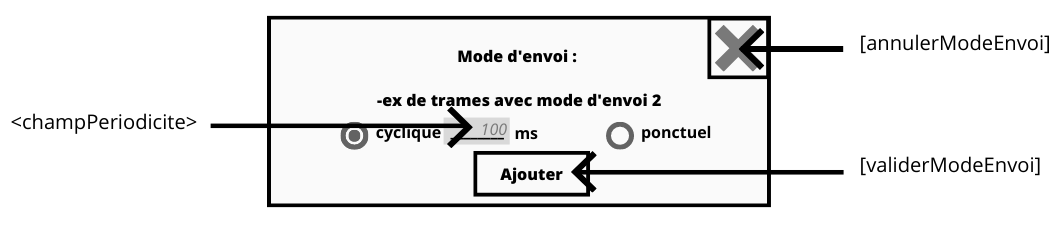
\includegraphics[width=0.93\textwidth]{sections/3_Exigences_specifiques/1_IHM/ihm/popUpTrame.png}
    \captionsetup{justification=centering, margin={1cm,0cm}}
    \captionof{figure}{PopupModeEnvoiTrame avec nom des boutons et du \newline champ de saisie de la périodicité}
    \label{ecran_mode_trame_envoi}
\end{minipage}\\ \\

\begin{minipage}{1.3\linewidth}
    \centering
    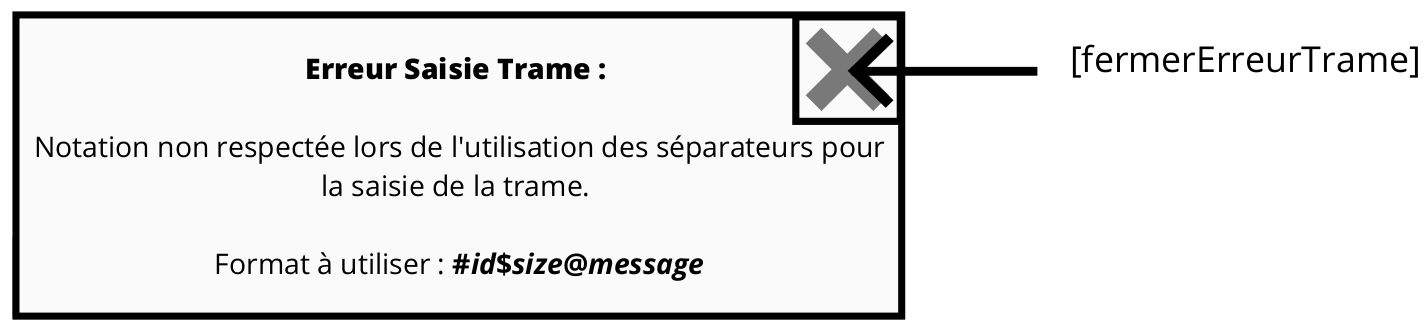
\includegraphics[width=0.66\textwidth]{sections/3_Exigences_specifiques/1_IHM/ihm/popUpErreurTrame.png}
    \captionsetup{justification=centering, margin={-5cm,0cm}}
    \captionof{figure}{PopupErreurSaisieTrame avec nom du bouton}
    \label{ecran_erreur_saisie_trame}
\end{minipage}\\ \\

\begin{minipage}{1.3\linewidth}
    \centering
    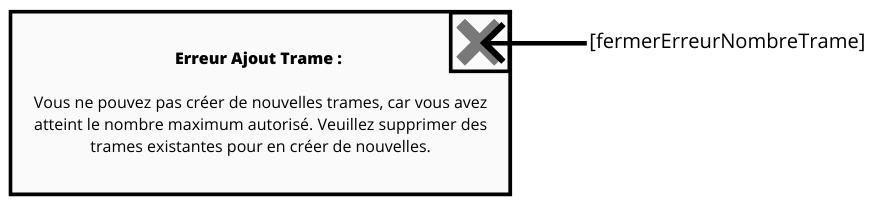
\includegraphics[width=0.66\textwidth]{sections/3_Exigences_specifiques/1_IHM/ihm/popUpErreurAjoutTrame.png}
    \captionsetup{justification=centering, margin={-5cm,0cm}}
    \captionof{figure}{PopupErreurNombreTrame avec nom du bouton}
    \label{ecran_erreur_ajout_nombre_trame}
\end{minipage}\\ \\

\begin{minipage}{1\linewidth}
    \centering
    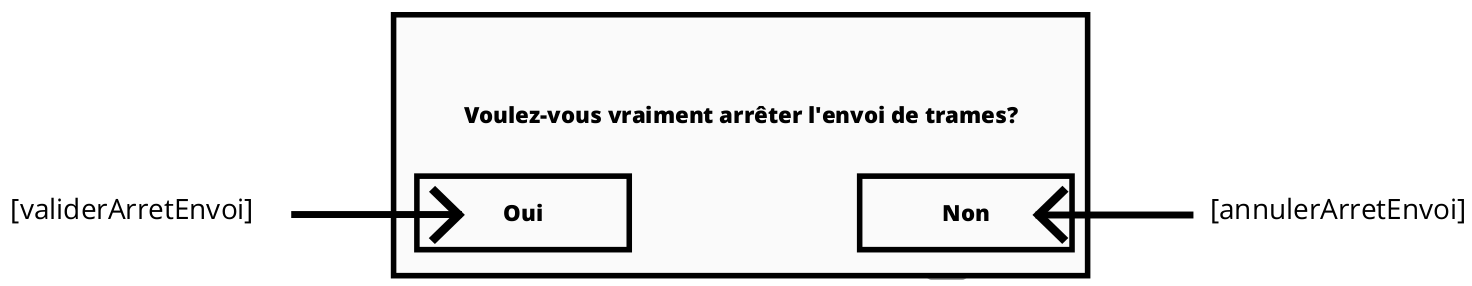
\includegraphics[width=0.91\textwidth]{sections/3_Exigences_specifiques/1_IHM/ihm/popUpArretEnvoi.png}
    \captionof{figure}{PopupArretEnvoi avec nom des boutons}
    \label{ecran_arret_envoi_trame}
\end{minipage}\\ \\

\begin{minipage}{1\linewidth}
    \centering
    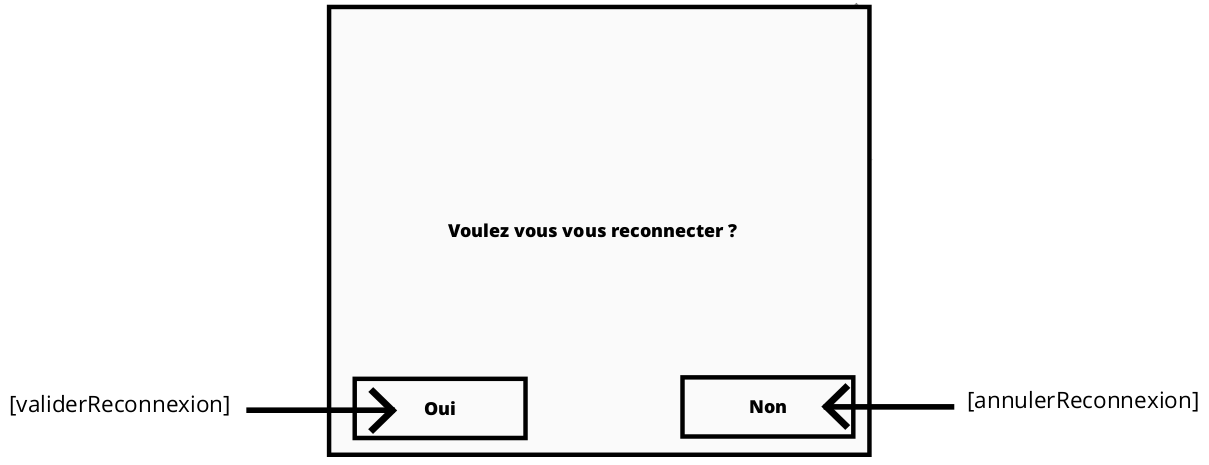
\includegraphics[width=0.9\textwidth]{sections/3_Exigences_specifiques/1_IHM/ihm/popUpReconnexion.png}
    \captionof{figure}{PopupDemandeReconnexion avec nom des boutons}
    \label{ecran_demande_reconnexion}
\end{minipage}\\ \\

\begin{minipage}{1\linewidth}
    \centering
    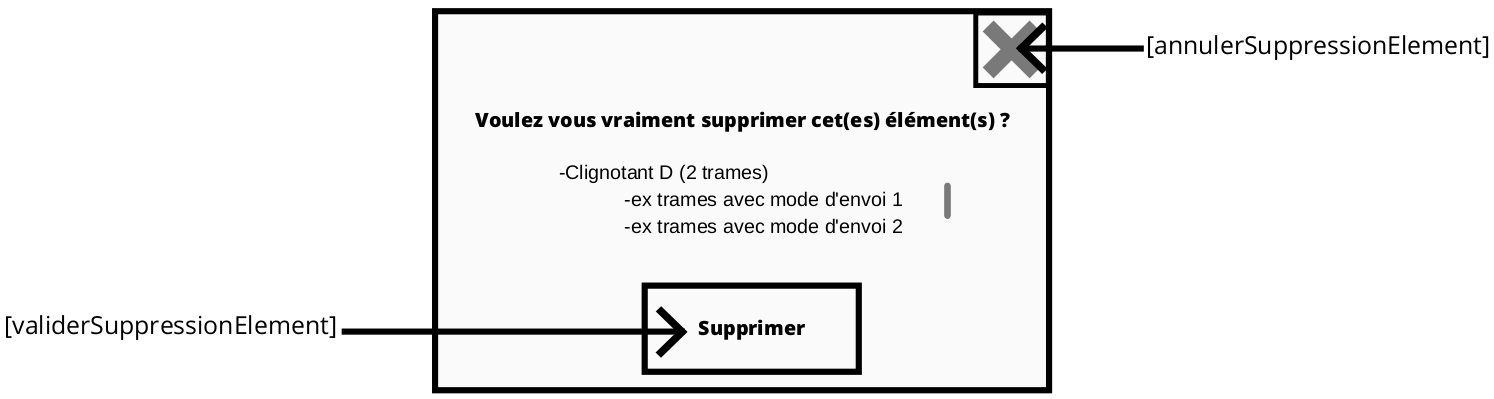
\includegraphics[width=0.9\textwidth]{sections/3_Exigences_specifiques/1_IHM/ihm/popUpSuppressionElementObjet.png}
    \captionof{figure}{PopupSuppressionElement avec nom des boutons}
    \label{ecran_suppression_element}
\end{minipage}\\